% ===========================================================================
% Chapter 6: Experiments 8 to 14
% Every number below is a registry value, a value printed in a cited paper, or
% an integer count. Registry keys are given in typewriter type.
% ===========================================================================
\chapter{Experiments 8 to 14}
\label{ch:exp814}

Chapter~\ref{ch:exp17} ended with one firm result: the same absorber has 7.34 times more
effect when it sits higher. This chapter compares that with spectral shape
(Experiment~8), lets the model's own chemistry place a candidate (Experiment~9), measures
how far two runs that should agree can differ (Experiment~10), and then tests published
spectra, every species the model can represent, iron minerals and ferric chloride
(Experiments~11 to~14). A change in the radiation field is measured as in
Section~\ref{sec:e7}, as a percentage of the reference field.

% ===========================================================================
\section{Experiment 8: spectral shape at a fixed placement}
\label{sec:e8}

\textbf{Question and design.} If the amount and height of the absorber are held fixed,
how much does the shape of its spectrum matter? Three runs put the spectra of ClS\sub{2}
(Experiment~8A), OSSO, that is S\sub{2}O\sub{2} (8B), and S\sub{3} (8C) in place of the
empirical spectrum, each scaled
so that its absorption added over 300 to 698~nm equals the empirical one, on the
unchanged profile. The optical depth of the absorber above 69~km is then 8.2458 for every
candidate (\texttt{spec\_8A.tau69}) against 8.1928 for the empirical spectrum
(\texttt{spec\_emp.tau69}), only 0.6461\% apart (\texttt{tau.spec\_change\_pct}). The runs
differ only in where along the wavelength axis the absorption sits.

\begin{figure}[tbp]
  \centering
  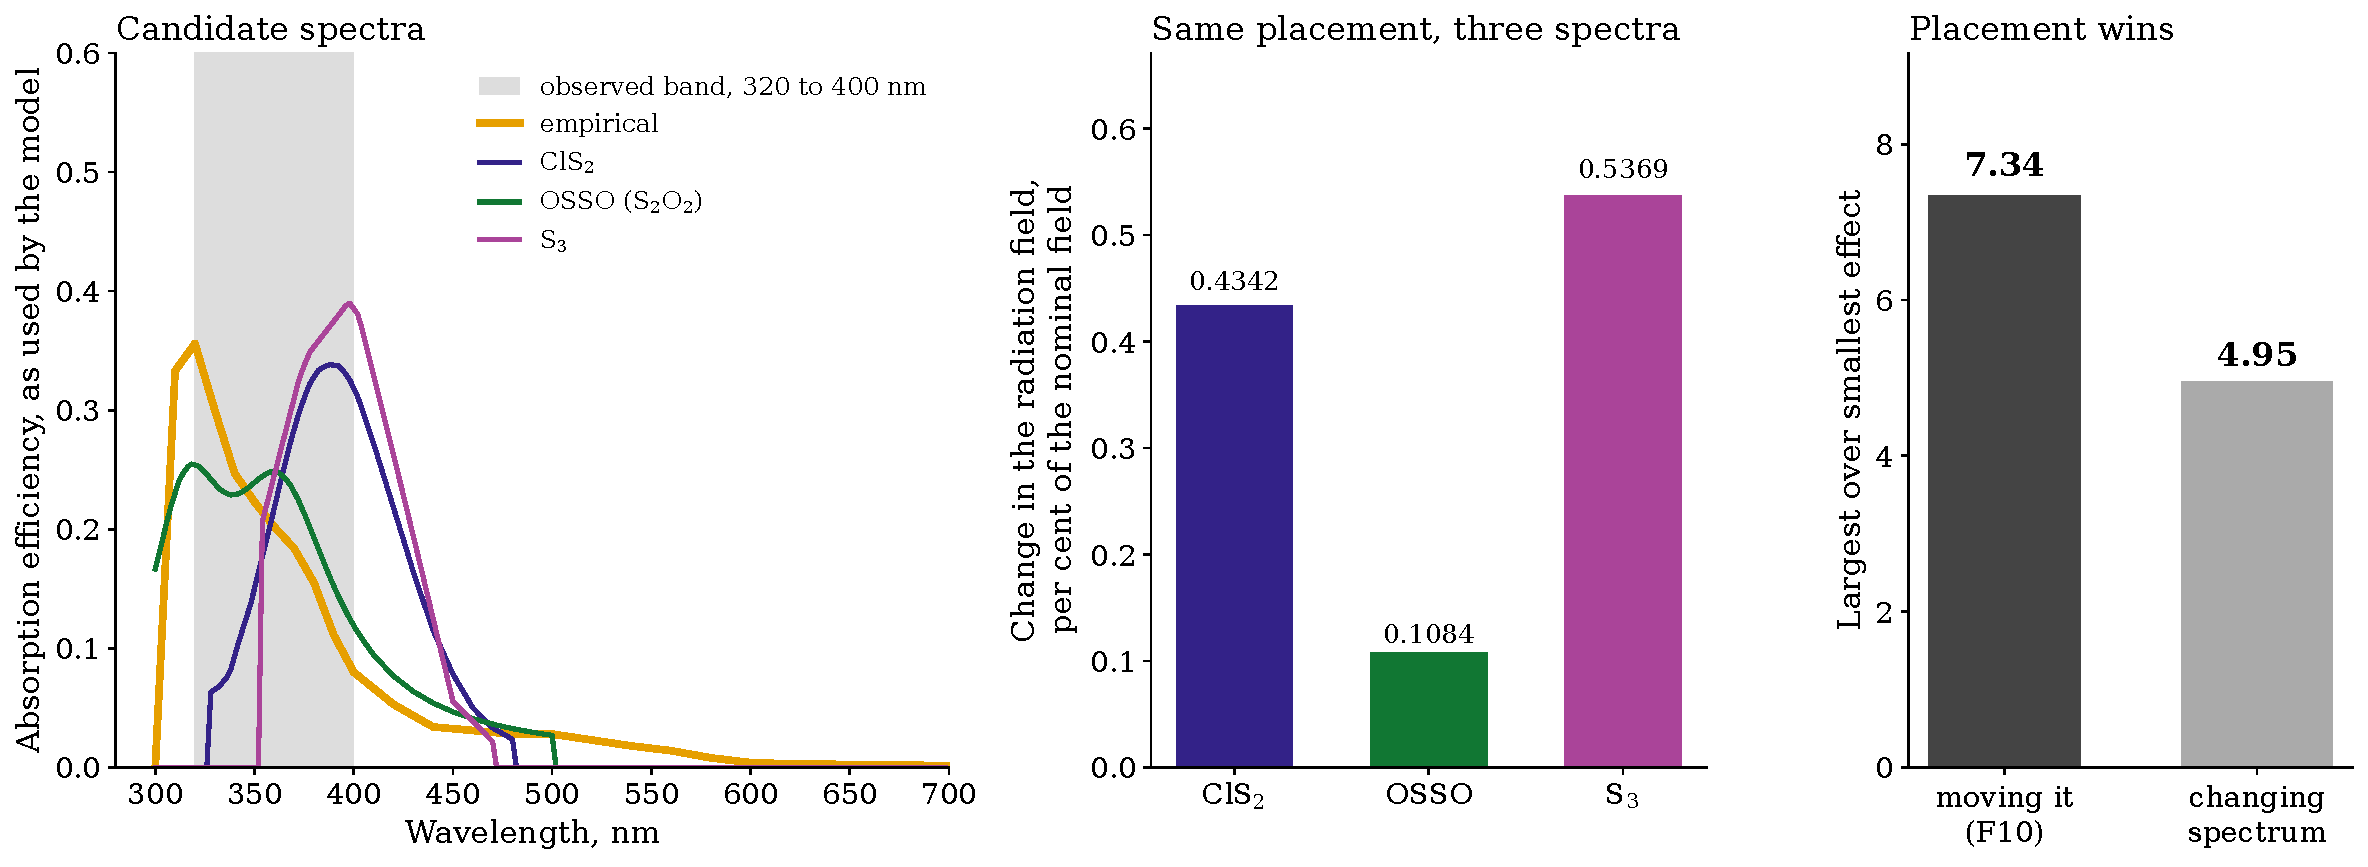
\includegraphics[width=0.92\textwidth]{F11_E08_spectrum-vs-placement_ch6_s12.pdf}
  \caption[Spectral shape against placement (Experiment~8)]{Spectral shape against placement (Experiment~8). Left: the spectra as the model
    uses them. Middle: change in the radiation field for each candidate at the same
    placement. Right: largest over smallest effect, for moving the absorber
    (Experiment~7) and for changing its spectrum. Keys \texttt{e8a.L2pct},
    \texttt{e8b.L2pct}, \texttt{e8c.L2pct}, \texttt{e7a.L2pct} and \texttt{e7b.L2pct}.}
  \label{fig:F11}
\end{figure}

\textbf{Result.} The radiation field changes by 0.4342\% for ClS\sub{2}, 0.1084\% for
OSSO and 0.5369\% for S\sub{3} (\texttt{e8a.L2pct}, \texttt{e8b.L2pct},
\texttt{e8c.L2pct}; Figure~\ref{fig:F11}). The largest is 4.95 times the smallest, so
spectral shape is a real, independent control. But moving the absorber changed the effect
7.34-fold, and the largest spectral effect is well below the 2.2498\% of the upward move.
\emph{Placement matters more than spectral shape, and spectral shape is not negligible.}
This comparison is the quantitative core of Phase~1. One caution: the responses are in the
reverse order of each spectrum's correlation with the empirical one, 0.9394 for OSSO,
0.3419 for ClS\sub{2} and 0.2253 for S\sub{3} (\texttt{corr.8B}, \texttt{corr.8A},
\texttt{corr.8C}). Since the empirical spectrum was fitted to the observed brightness of
Venus, the ranking measures resemblance to that fit, not correctness.

\textbf{The amount check.} A script that only reads the saved baseline divided the
required optical depth $\tau_{\mathrm{req}}$ (Section~\ref{sec:taureq}) by the optical
depth that each of twelve sulfur and chlorine species gives with its column above 58~km,
at the wavelength where its absorption peaks within 300 to 620~nm. The result, the
\emph{shortfall factor},
is how many times too little of the species there is. ClS\sub{2} comes closest, short by
121.914 at 388~nm (\texttt{scr.ClS2.short}), about two orders of magnitude; next is
S\sub{2}O at 6070, and the rest are short by $4.4\times10^{4}$ (\texttt{scr.S2.short}) to
$4.2\times10^{8}$ (\texttt{scr.SCl.short}). OSSO is short by $4.2\times10^{6}$
(\texttt{scr.S2O2.short}). Egan et al.\ found OSSO about three orders of magnitude too low
by a different route~\cite{egan2025osso}. The two agree in direction and differ in size
because they measure against different things, and theirs uses SO\sub{2} above the clouds
kept deliberately high to give OSSO every chance~\cite{egan2025osso}. OSSO is the only
candidate with an independent published verdict, so this agreement is the main outside
check on the screen's arithmetic. ClS\sub{2}, the one species close in amount, went
forward to Experiment~9. Table~\ref{tab:scr} lists all twelve.

\begin{table}[htbp]
  \centering
  \caption[The amount check (Experiment~8)]{The amount check of Experiment~8: each species' column above 58~km, at the
    wavelength where its absorption peaks within 300 to 620~nm, against the required
    optical depth. Keys
    \texttt{scr.<species>.lam} and \texttt{scr.<species>.short}.}
  \label{tab:scr}
  \footnotesize
  \setstretch{1.0}
  \begin{tabular}{lcc}
    \toprule
    Species & Peak wavelength (nm) & Shortfall factor \\
    \midrule
    ClS\sub{2} & 388 & $1.219\times10^{2}$ \\
    S\sub{2}O & 300 & $6.070\times10^{3}$ \\
    S\sub{2} & 300 & $4.415\times10^{4}$ \\
    S\sub{3} & 398 & $7.486\times10^{4}$ \\
    S\sub{4} & 500 & $9.962\times10^{4}$ \\
    ClO & 300 & $6.754\times10^{5}$ \\
    SCl\sub{2} & 338 & $8.049\times10^{5}$ \\
    S\sub{2}Cl\sub{2} & 300 & $1.092\times10^{6}$ \\
    Cl\sub{2} & 328 & $1.604\times10^{6}$ \\
    OSSO & 318 & $4.207\times10^{6}$ \\
    SO\sub{3} & 300 & $8.626\times10^{6}$ \\
    SCl & 470 & $4.205\times10^{8}$ \\
    \bottomrule
  \end{tabular}
\end{table}

% ===========================================================================
\section{Experiment 9: letting the chemistry place the candidate}
\label{sec:e9}

\textbf{Question and design.} Experiments~7 and~8 used the empirical profile, a height
chosen by the modeller. What happens when a candidate sits where the model's own
chemistry puts it? The ClS\sub{2} spectrum was kept, and the absorber profile was given
the shape of the model's own steady-state ClS\sub{2} profile, rescaled so that the sum of
the absorber over all levels stayed the same. The expected outcome was written down
before the run: if the absorber left the response band, the run should reproduce the
difference between the runs with and without the absorber (Section~\ref{sec:e6}), with
the opposite sign.

\begin{figure}[tbp]
  \centering
  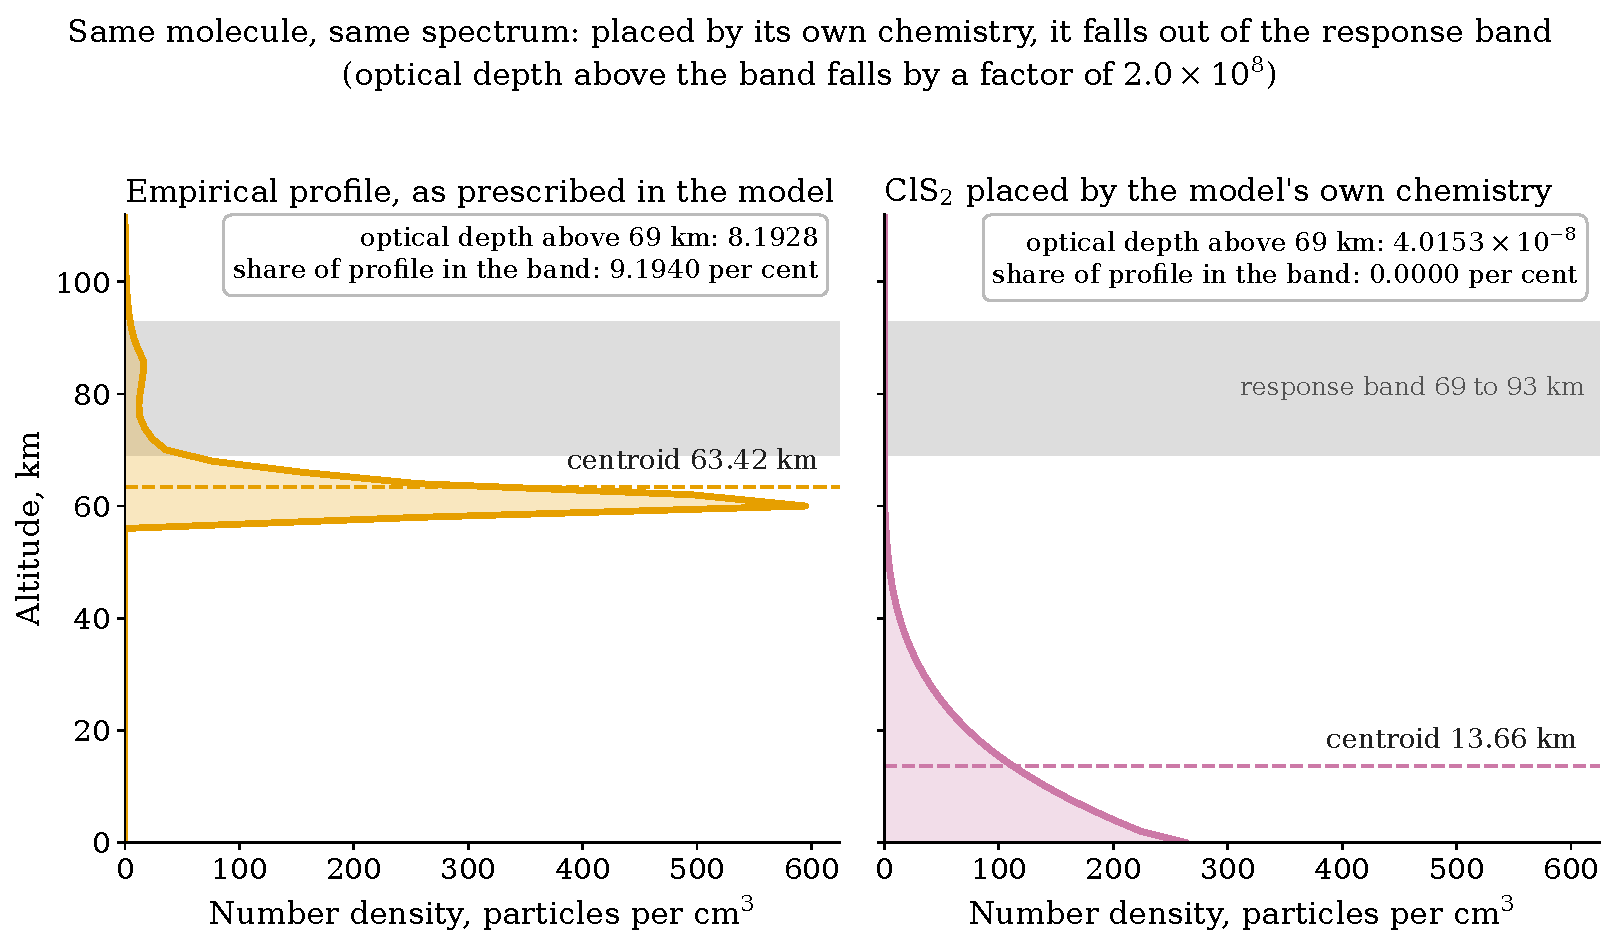
\includegraphics[width=0.8\textwidth]{F12_E09_ClS2-self-placement_ch6_s13.pdf}
  \caption[The same molecule and spectrum, placed two ways (Experiment~9)]{The same molecule and spectrum, placed two ways (Experiment~9). Left: the
    empirical profile. Right: the profile the model's own chemistry gives ClS\sub{2}. The
    grey band is the response band. Keys \texttt{pnom.centroid}, \texttt{p9.centroid},
    \texttt{spec\_emp.tau69}, \texttt{spec\_9.tau69}, \texttt{pnom.inband},
    \texttt{p9.inband} and \texttt{tau.reduction}.}
  \label{fig:F12}
\end{figure}

\textbf{Where the chemistry puts it.} The empirical absorber is a layer at the cloud top,
centred at 63.419~km (\texttt{pnom.centroid}), with 9.1940\% of its column inside the
response band (\texttt{pnom.inband}). The model's ClS\sub{2} is centred at 13.656~km
(\texttt{p9.centroid}), 51.521~km lower (\texttt{e9.centroid\_shift}), with 91.80\% of it
below 30~km (\texttt{p9.below30}) and 0.0000\% inside the band (\texttt{p9.inband};
Figure~\ref{fig:F12}). The registry shows where the chemistry puts it, not why; how fast
ClS\sub{2} is made and destroyed at each height is the quantity Phase~2 measures first
(Chapter~\ref{ch:phase2}, WP5). The optical depth above 69~km
falls from 8.1928 to $4.0153\times10^{-8}$ (\texttt{spec\_9.tau69}), a factor of
$2.0\times10^{8}$ (\texttt{tau.reduction}). Keeping the level sum fixed left the column
(Section~\ref{sec:conv-col}) 12.88\% lower (\texttt{p9.col\_deficit\_pct}), because the
new profile puts that share of its level sum in the model's lowest layer, which is only
2~cm thick; beside a factor of $2.0\times10^{8}$ this cannot matter.

\textbf{Result.} The prediction held. The peak change in actinic flux has the size and
place of the no-absorber control, at 81~km and 328~nm, with the opposite sign. Added cell
by cell, the two change fields leave 0.001487\% of the control
(\texttt{id.l2\_ratio\_pct}), and over the 3425 cells carrying more than 1\% of the peak
their ratio has mean 0.99994 and standard deviation $9.4\times10^{-5}$
(\texttt{id.ratio\_mean}, \texttt{id.ratio\_sd}).

\emph{This is the central result of Phase~1.} Placed where the model's own chemistry puts
it, ClS\sub{2} is radiatively the same as no absorber at all in the band where the
absorber acts. It is in the calculation at full strength, with a spectrum in the right
range, but in the wrong place. A candidate can come close in amount and have a suitable
spectrum and still be invisible, because the chemistry places it below the altitudes where
the radiation responds. This failure is separate from its shortfall in amount.

The two photolysis conventions of Section~\ref{sec:conv-J} give different pictures here,
and both are correct. Nearly every rate coefficient rises a little, the largest
$\Delta J$ being 3.168\% for S\sub{2}O\sub{2} at 81~km (\texttt{dJ.e9.S2O2}); those of
SO\sub{2} and SO fall very slightly (\texttt{dJ.e9.SO2}, \texttt{dJ.e9.SO}). But the rate
$\Delta(Jn)$ of S\sub{2}Cl\sub{2} and SCl\sub{2} photolysis falls by 21.751\% and
19.630\% at 69~km (\texttt{dJy.e9.S2Cl2}, \texttt{dJy.e9.SCl2}). Since the coefficients
rise, these falls come from smaller amounts of the two molecules, and those amounts are
abundances, which the floor of Section~\ref{sec:conv-floor} limits; no cause is claimed
for them. The largest change among the sulfur reservoirs in the band, SO by 0.7384\%
(\texttt{res.e9.SO.inband}), is below that floor, so no abundance result is claimed.

% ===========================================================================
\section{Experiment 10: a replicate, two floors and a retraction}
\label{sec:e10}

Experiment~10 put the S\sub{3} spectrum on the same ClS\sub{2} profile, to test whether a
pattern seen in Experiment~9 held for a third combination. The test was void: both
spectra lie wholly inside the range used for scaling and were scaled to the same total on
the same profile, so the optical depth above 69~km is identical to every digit kept
(\texttt{tau.9\_minus\_10} is zero), and the difference between the two actinic flux
fields is only 0.0017\% of the change that Experiment~9 makes
(\texttt{e10.fielddiff\_pct}; Section~\ref{sec:conv-field}). Experiment~10 is a numerical replicate of
Experiment~9, and that accident gave three results.

\begin{figure}[tbp]
  \centering
  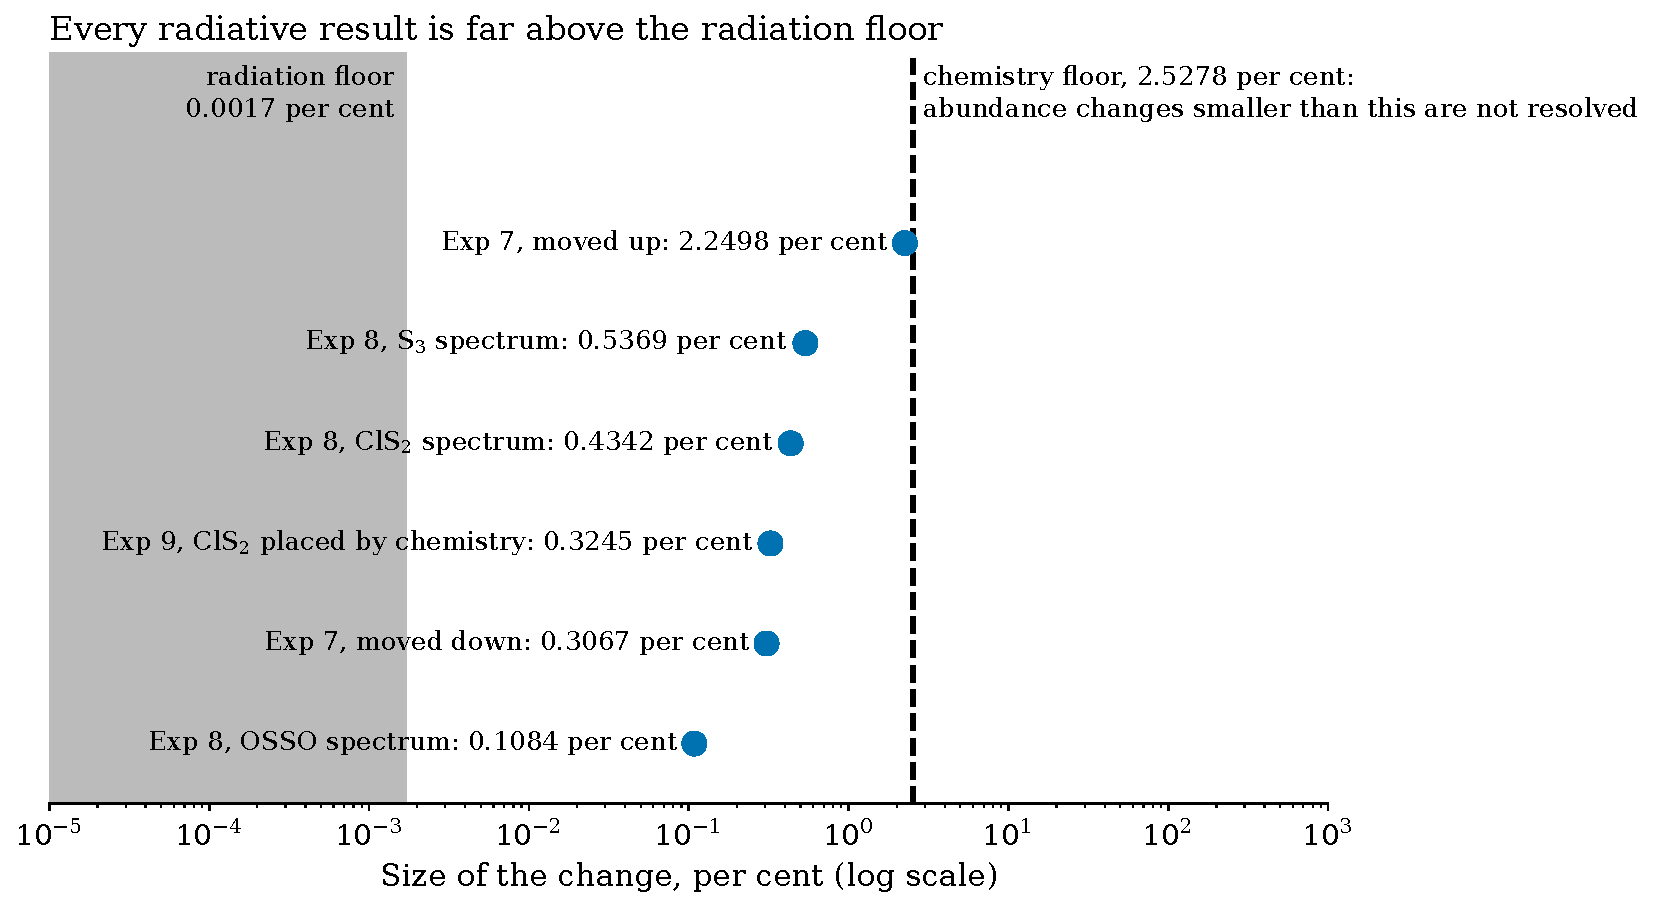
\includegraphics[width=0.8\textwidth]{F13_E10_noise-floors_ch6_backup.pdf}
  \caption[The two floors (Experiments~9 and~10)]{The two floors (Experiments~9 and~10). Every radiative result lies far above
    the radiation floor of 0.0017\% (\texttt{e10.fielddiff\_pct}), which is a share of the
    change Experiment~9 makes and so smaller still as a share of the field; the chemistry
    floor of 2.5278\% (\texttt{res.e10.SO.inband}) applies to abundances only.}
  \label{fig:F13}
\end{figure}

\textbf{Two floors, not one.} Since the radiation fields agree, any difference in the
chemistry is numerical. SO in the band differs from the baseline by 0.7384\% in one run
and 2.5278\% in the other (\texttt{res.e10.SO.inband}): this is the chemistry floor of
Section~\ref{sec:conv-floor}. Figure~\ref{fig:F13} sets it beside the radiation floor of
0.0017\%. The two numbers are not on the same footing. Every radiative result, from
0.1084\% for OSSO to 2.2498\% for the upward move, is a share of the field
(Equation~\eqref{eq:field}); the radiation floor is a share of the change Experiment~9
makes, and that change is itself only 0.3245\% of the field (\texttt{e9.L2pct}). Two runs
that should agree therefore differ by far less than any result, so every radiative
comparison stands; the chemistry floor limits only claims about abundances. Only two abundance changes in the
project exceed it clearly: those of SO and SO\sub{3} when the absorber is moved up
(Section~\ref{sec:e7}); SO also crosses it narrowly in Experiments~3 and~4B.

\textbf{Spectral shape matters only where the absorber overlaps the responding layer.}
On the empirical profile, S\sub{3} gives 1.2365 times the effect of ClS\sub{2}; on the
ClS\sub{2} profile the same ratio is 1.000003. Out of the band, the spectrum no longer
matters (keys \texttt{twoby2.nominal\_ratio} and \texttt{twoby2.cls2\_ratio}).

\textbf{A retraction.} In Experiment~9 the change in each of nine photolysis rate
coefficients was the change in Experiment~7B times one constant, 1.0474 with standard
deviation 0.00056 (\texttt{chr.mean}, \texttt{chr.sd}); the nine ratios are ClS\sub{2} 1.0473, H\sub{2}SO\sub{4} 1.0466, S\sub{2}Cl\sub{2} 1.0482, S\sub{2}O 1.0480, OSSO 1.0477, S\sub{3} 1.0472, S\sub{4} 1.0466, SCl 1.0469, SCl\sub{2} 1.0477 (keys \texttt{chr.<species>}). This had been read as a
``fingerprint'' of absorbers below the cloud top. It is not: the ratio of the actinic flux
changes themselves at 81~km, the peak response height, added over all wavelengths, is
1.0473 (\texttt{chr.flux\_ratio}). The constant is linear response; when two small disturbances
change the light in the same place, every photolysis rate follows the light. For
Experiment~7A, where the optical depth above 69~km is 10.1975 times the nominal
(\texttt{tau.7A\_over\_A1}), the ratios for eight of the species scatter widely (mean $-14.12$, spread 12.43;
\texttt{chr8\_7a\_7b.mean} and \texttt{.spread}),
which locates the edge of the linear regime. The fingerprint reading is withdrawn in
commit \texttt{5a7e2ac}.

% ===========================================================================
\section{Experiment 11: computed cross sections of two isomers}
\label{sec:e11}

\textbf{Question and design.} Trabelsi and Francisco computed the cross sections of two
chlorine and sulfur isomers, ClSSCl and SSCl\sub{2}, and offer them as model
inputs~\cite{trabelsi2026}; the model tracks only one lumped species, S\sub{2}Cl\sub{2}.
The computed data, obtained from the authors and checked against their published figure,
were run as absorber spectra under the rules of Experiment~8, SSCl\sub{2} in
Experiment~11A and ClSSCl in 11B.

\begin{figure}[tbp]
  \centering
  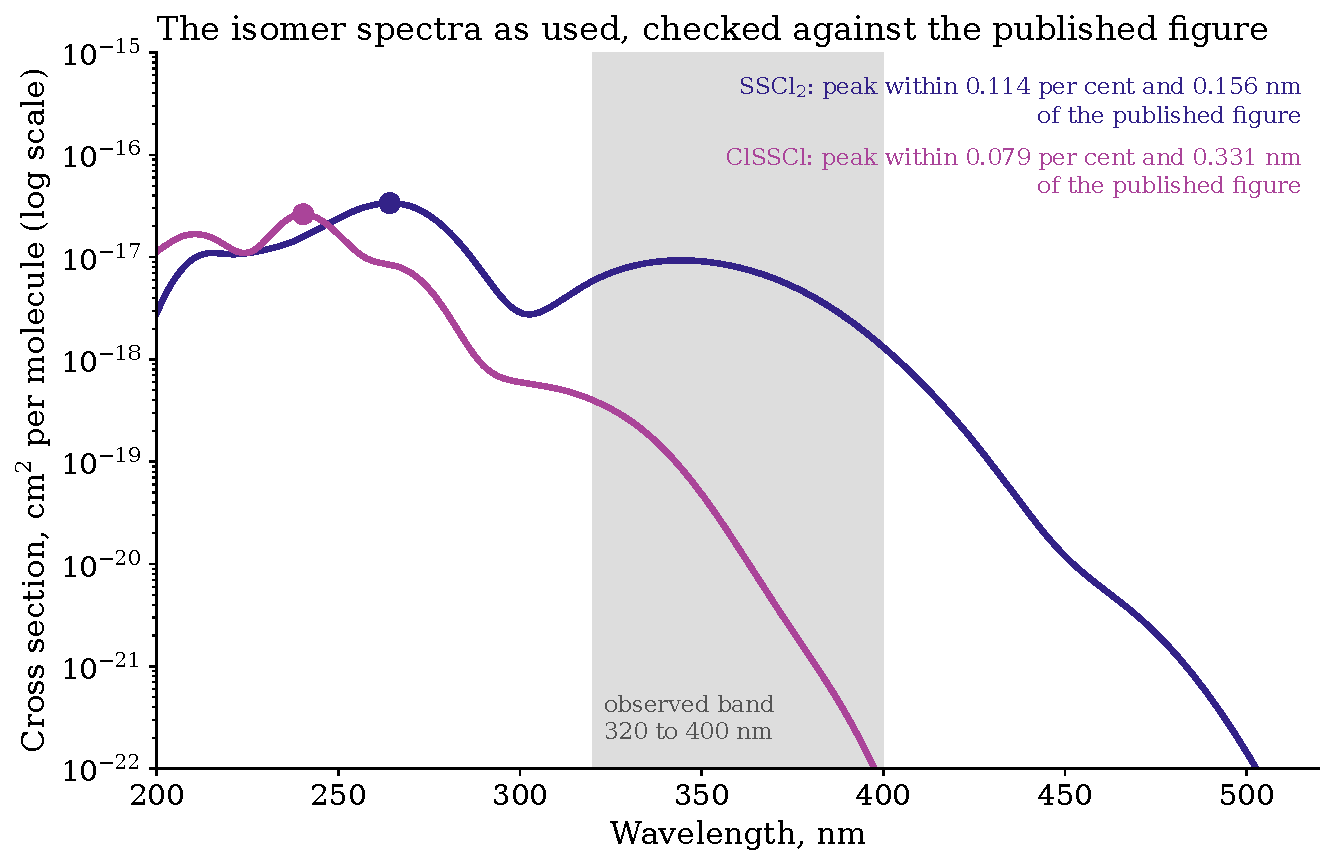
\includegraphics[width=0.66\textwidth]{F14_E11_published-cross-sections_ch6_report.pdf}
  \caption[The isomer cross sections as used, checked against the published figure (Experiment~11)]{The isomer cross sections as used, checked against the published figure
    (Experiment~11). Keys \texttt{iso.SSCl2.val\_pct}, \texttt{iso.SSCl2.val\_nm},
    \texttt{iso.ClSSCl.val\_pct} and \texttt{iso.ClSSCl.val\_nm}.}
  \label{fig:F14}
\end{figure}

\textbf{Result.} Each peak matches the published figure to 0.114\% in height and
0.156~nm in position for SSCl\sub{2}, and 0.079\% and 0.331~nm for ClSSCl
(Figure~\ref{fig:F14}). SSCl\sub{2} puts 85.49\% of its absorption between 320 and
400~nm, more than any other spectrum tested and more than the empirical 61.58\%; its
correlation with the empirical spectrum, 0.88983, is second to OSSO's (keys
\texttt{share320400.11A}, \texttt{share320400.emp} and \texttt{corr.11A}). It is therefore the best
match by share but only the second by correlation. On the empirical profile
the field changes by 0.19465\% for SSCl\sub{2} and 0.30144\% for ClSSCl
(\texttt{e11a.L2pct}, \texttt{e11b.L2pct}). Across all five spectra the responses fall in
exactly the reverse order of their correlations (rank correlation $-1$,
\texttt{five.spearman}), with the caution of Experiment~8.

Neither isomer can be made in the amount needed: at its absorption peak within 300 to
620~nm SSCl\sub{2} is short
by $4.266\times10^{5}$ and ClSSCl by $6.668\times10^{6}$ (\texttt{iso.SSCl2.short},
\texttt{iso.ClSSCl.short}). ClSSCl absorbs most strongly near 240~nm, below the start of
the absorber's grid at 300~nm, so the model sees only its tail, scaled up to a peak
efficiency of 0.9467 against the empirical 0.356 (\texttt{spec\_11B.peakQ}); its response
describes that tail, not the molecule. Within the literature reviewed in
Chapter~\ref{ch:lit}, no earlier study has run computed chlorine and sulfur cross sections
in a Venus photochemistry model; this is the extent of the review, not a certainty.

% ===========================================================================
\section{Experiment 12: all three tests on every species}
\label{sec:screen}

\textbf{Question and design.} Which species the model can represent pass amount,
placement and spectrum together? A read-only script scored every species in the network
with a cross section between 300 and 620~nm: 23 of the 62 tracked
(\texttt{e12.n\_screened}, \texttt{e12.n\_tracked}). Nineteen have no cross section in
that range, 18 have none at all, and the two cloud particle tracers are excluded; a
species absent from the network, such as ferric chloride, cannot be screened. Two choices,
learned from Experiment~9, differ from the Experiment~8 check. A species is credited only
with its column \emph{above 69~km}, and it is compared with the absorber \emph{at each
wavelength}, not at its own peak, which would favour species whose absorption falls
steeply from below 300~nm. SO\sub{2} shows why: at its own peak it looks only 2.402 times
short above 58~km (\texttt{e12.SO2.shortfall58}), but at 360~nm above 69~km it is short by
4768.6 (\texttt{e12.SO2.short.360}). ClS\sub{2} goes from 121.914 to $8.0\times10^{6}$
(\texttt{e12.ClS2.short.360}), because almost none of it is above 69~km.

The screen itself sets no pass marks. The marks used here (Figure~\ref{fig:F3}) are set so
that the empirical absorber itself passes every test: a shortfall at 360~nm of at most 1,
which the absorber meets exactly; at least the absorber's own 11.92\% of the column above
58~km inside the band (\texttt{e12.gate.emp\_inband\_pct}); and more than half of the
absorption inside 320 to 400~nm, with a correlation above 0.5.

\begin{figure}[tbp]
  \centering
  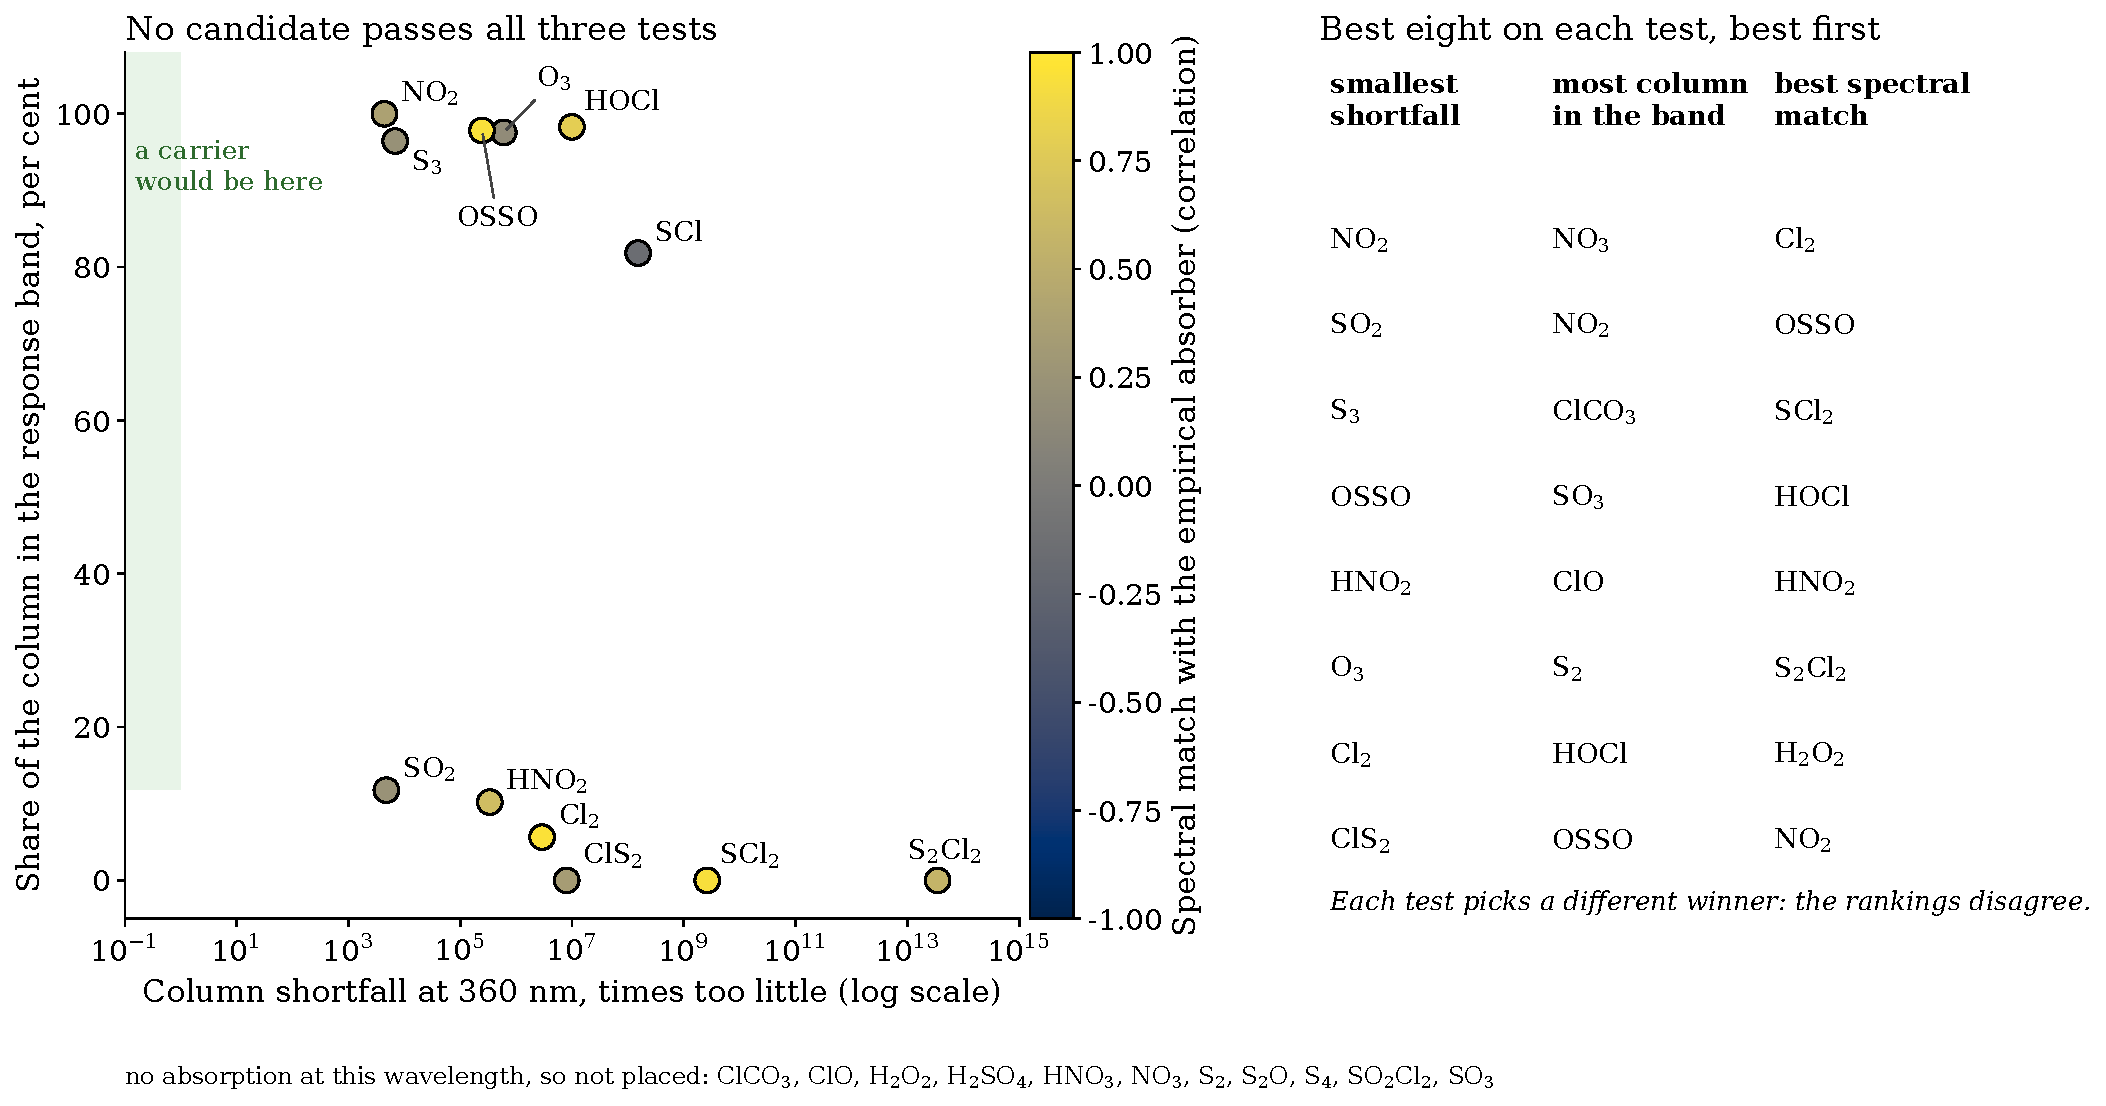
\includegraphics[width=\textwidth]{F15_E12_three-axis-screen_ch6_s14.pdf}
  \caption[The three-axis screen (Experiment~12)]{The three-axis screen (Experiment~12): shortfall at 360~nm (horizontal), share
    of the column in the response band (vertical) and spectral correlation (colour). A
    carrier would sit in the shaded corner, with no shortfall and most of its column in
    the band; species that do not absorb at 360~nm are listed below the axis. The right
    panel lists the best eight species on each test. Keys \texttt{e12.X.short.360},
    \texttt{e12.X.frac\_in\_band\_pct} and \texttt{e12.X.corr}, where X is the species.}
  \label{fig:F15}
\end{figure}

\textbf{Result.} Table~\ref{tab:screen} gives every species. Sixteen species pass on
placement and five on spectrum. Two pass both, OSSO
and HOCl, yet in amount they are short by $2.4563\times10^{5}$ and $9.9572\times10^{6}$. None passes on amount, so none passes all three
(Figure~\ref{fig:F15}; keys \texttt{e12.gate.n\_placement}, \texttt{e12.gate.n\_spectrum},
\texttt{e12.gate.n\_all}, \texttt{e12.S2O2.short.360} and \texttt{e12.HOCl.short.360}). The tests also
disagree about which species is ``best''. NO\sub{2} is the least short, by a factor of
4402.887 (key \texttt{e12.best\_shortfall}), and has 99.998\% of its column in the band, but peaks at
430~nm with a correlation of only 0.3862. HNO\sub{2} has the most absorption inside 320 to
400~nm, 98.031\%, but only 10.216\% of its column in the band. Cl\sub{2} correlates best,
at 0.9461, with 5.647\% in the band. No single ``most likely'' ranking exists.

\begin{table}[htbp]
  \centering
  \caption[The three-axis screen for all 23 species (Experiment~12), ordered by shortfall]{The three-axis screen for all 23 species (Experiment~12), ordered by shortfall.
    Shortfall: times too little at 360~nm above 69~km (``none at 360~nm'': the species does
    not absorb there). In band: per cent of the column above 58~km that lies in the
    response band. Share: per cent of the absorption between 300 and 698~nm that lies in
    320 to 400~nm. Pass marks: shortfall at most 1; in band at least 11.92 per cent; share
    above 50 per cent with correlation above 0.5. Keys \texttt{e12.<species>.short.360},
    \texttt{.frac\_in\_band\_pct}, \texttt{.share\_320\_400\_pct}, \texttt{.corr} and
    \texttt{e12.gate.*}.}
  \label{tab:screen}
  \footnotesize
  \setstretch{1.0}
  \begin{tabular}{lccccl}
    \toprule
    Species & Shortfall & In band (\%) & Share (\%) & Correlation & Passes on \\
    \midrule
    NO\sub{2} & $4.403\times10^{3}$ & 99.998 & 36.140 & $0.386$ & placement \\
    SO\sub{2} & $4.769\times10^{3}$ & 11.772 & 4.272 & $0.239$ & none \\
    S\sub{3} & $6.859\times10^{3}$ & 96.447 & 56.926 & $0.225$ & placement \\
    OSSO & $2.456\times10^{5}$ & 97.835 & 64.275 & $0.939$ & placement, spectrum \\
    HNO\sub{2} & $3.384\times10^{5}$ & 10.216 & 98.031 & $0.646$ & spectrum \\
    O\sub{3} & $6.012\times10^{5}$ & 97.570 & 5.606 & $0.169$ & placement \\
    Cl\sub{2} & $2.910\times10^{6}$ & 5.647 & 73.719 & $0.946$ & spectrum \\
    ClS\sub{2} & $8.010\times10^{6}$ & $1.3\times10^{-4}$ & 60.673 & $0.342$ & none \\
    HOCl & $9.957\times10^{6}$ & 98.295 & 52.967 & $0.796$ & placement, spectrum \\
    SCl & $1.523\times10^{8}$ & 81.836 & 14.474 & $-0.156$ & placement \\
    SCl\sub{2} & $2.618\times10^{9}$ & $2.3\times10^{-3}$ & 71.043 & $0.936$ & spectrum \\
    S\sub{2}Cl\sub{2} & $3.469\times10^{13}$ & $5.0\times10^{-6}$ & 32.933 & $0.570$ & none \\
    ClCO\sub{3} & none at 360~nm & 99.981 & 0 & $0.225$ & placement \\
    ClO & none at 360~nm & 99.332 & 4.121 & $0.159$ & placement \\
    H\sub{2}O\sub{2} & none at 360~nm & 58.857 & 27.559 & $0.484$ & placement \\
    H\sub{2}SO\sub{4} & none at 360~nm & 0.969 & 0 & $-0.218$ & none \\
    HNO\sub{3} & none at 360~nm & 34.902 & 6.619 & $0.215$ & placement \\
    NO\sub{3} & none at 360~nm & 100.000 & 0 & $-0.519$ & placement \\
    S\sub{2} & none at 360~nm & 98.741 & 0.167 & $0.253$ & placement \\
    S\sub{2}O & none at 360~nm & 50.181 & 4.159 & $0.239$ & placement \\
    S\sub{4} & none at 360~nm & 97.261 & 0 & $-0.304$ & placement \\
    SO\sub{2}Cl\sub{2} & none at 360~nm & 35.317 & 0 & $-0.039$ & placement \\
    SO\sub{3} & none at 360~nm & 99.847 & 10.286 & $0.314$ & placement \\
    \bottomrule
  \end{tabular}
\end{table}

Amount is a gate, not a tie-breaker: the shortfalls run from thousands to about $10^{13}$,
while placement and spectrum were each worth less than a factor of ten.

% ===========================================================================
\section{Experiment 13: iron and sulfur minerals}
\label{sec:e13}

\textbf{Question and design.} Jiang et al.\ proposed rhomboclase and acid ferric sulfate
from their spectral shape~\cite{jiang2024}. Spacek et al.\ later derived how strongly the
droplet liquid must absorb: a decadic coefficient of 1278 per centimetre at
375~nm~\cite{spacek2026}. Nobody had put the two together. Using the mass extinction
coefficients measured by Jiang et al.\ and the straight-line scaling of Spacek et al., the
mass of mineral needed per litre of droplet is the requirement divided by the coefficient:
\begin{equation}
  m = \frac{a_{\mathrm{req}}}{\varepsilon} , \qquad s = 100\,\frac{m}{\rho} ,
  \label{eq:loading}
\end{equation}
where $a_{\mathrm{req}} = 1278$ per centimetre is the required decadic coefficient at
375~nm (\texttt{e13.A\_required}), $\varepsilon$ is the material's mass absorption
coefficient at 375~nm in square centimetres per gram, $m$ is the mass needed in grams per
cubic centimetre, which is the same number in kilograms per litre, and $s$ is that mass
as a share of the 1.8~kg that a litre of droplet liquid weighs, the droplet density used
by Dai et al.~\cite{dai2023kzz} (\texttt{e13.rho\_solution}).
For rhomboclase $\varepsilon$ is 422.797 and for acid ferric sulfate 293.144
(\texttt{e13.X.eps\_375}); for ferric chloride in water, 1~g per litre gives about 1 per
centimetre, so $\varepsilon$ is 1000.
The script first reproduces the ferric chloride figure of Spacek et al.\ from their
stated input, 1.278 against their 1.3~kg per litre (\texttt{e13.fecl3.loading\_kg\_per\_L});
that line is a check on the method, never a result about ferric chloride.

\begin{figure}[tbp]
  \centering
  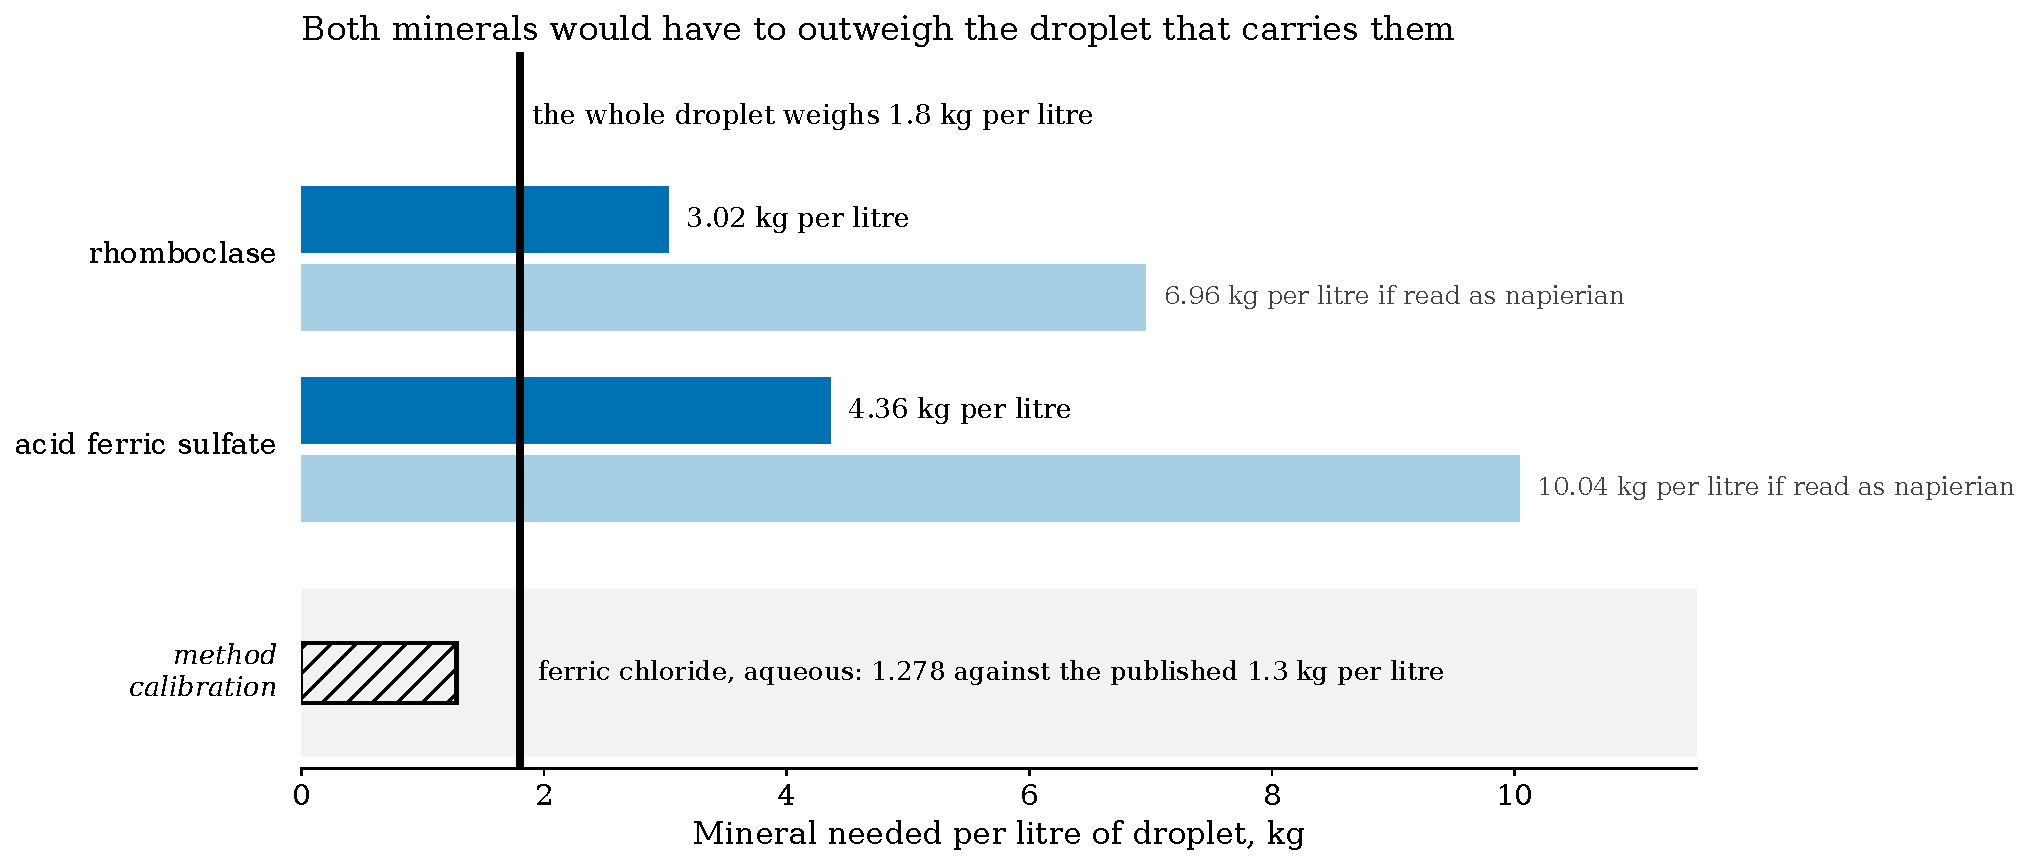
\includegraphics[width=0.9\textwidth]{F16_E13_minerals-cannot-reach_ch6_s15.pdf}
  \caption[Mineral needed per litre of droplet (Experiment~13)]{Mineral needed per litre of droplet to meet the requirement at 375~nm
    (Experiment~13); dark bars read the coefficients as decadic, light bars as natural
    (Napierian), the vertical line is the mass of a litre of droplet and the hatched
    bar is the calibration. Keys \texttt{e13.rhomboclase.*},
    \texttt{e13.acid\_ferric\_sulfate.*} and \texttt{e13.fecl3.*}.}
  \label{fig:F16}
\end{figure}

\textbf{Result.} Rhomboclase would need 3.02~kg per litre, 167.93\% of the droplet's own
mass, and acid ferric sulfate would need 4.36~kg per litre, 242.20\% (keys
\texttt{e13.X.pct\_of\_droplet}, where X is the mineral), against a droplet
density of 1.8~kg per litre (Figure~\ref{fig:F16}). At 375~nm, even a droplet made
entirely of either mineral could not absorb enough. Reading the coefficients as natural
rather than decadic raises the need to 6.96 and 10.04~kg per litre. At each mineral's own
absorption peak the need is 156.43\% and 95.07\% of the droplet mass
(\texttt{e13.X.pct\_at\_peak}): rhomboclase still cannot reach it, and acid ferric sulfate
could only as a droplet almost wholly made of the mineral.
The verdict is also conservative: the coefficients were measured through a suspension and
include scattering, and removing it can only raise the mass needed.

% ===========================================================================
\section{Experiment 14: ferric chloride measured in acid}
\label{sec:e14}

Experiment~14 was done after Phase~1 closed; it is reported because it changes how a
published result should be read.

\textbf{Question and design.} Spacek et al.\ find the absorbance of ferric chloride too
low, because it would need about 1.3~kg per litre~\cite{spacek2026}; the method of
Experiment~13 gives 1.278~kg per litre from the same input, which with the droplet density
is 71.0\% of the droplet mass (\texttt{e14.aqueous\_pct\_of\_droplet}). Their input
is an absorbance measured in water. Egan et al.\ note that the solvent has a significant
effect on the spectrum of ferric chloride, and derived its molar absorptivity in
hydrochloric acid at five strengths, from 1.54 to 12.2 moles per litre, labelling the
curves Cl~A to Cl~E; they use these curves as the ferric chloride components when they
fit their mixed sulfuric and hydrochloric acid samples~\cite{egan2025lab}. One script read those five curves
from the published figure at 600 dots per inch and writes nothing unless three checks
pass. The first finds the frame of the left panel, so that every point is measured from
the true axes. The second requires the tick marks to be evenly spaced to better than
1\% on both axes, so that the scale has been read without stretching. The third requires
every curve to fall back to zero at its long-wavelength end, so that the vertical zero is
where the figure puts it. To test the checks, the zero was deliberately shifted; the
third check first let the shift through, and was tightened to a tenth of a tick until it
caught it. A second script reproduces the figure of Spacek et al.\ from their aqueous input,
1.278 against their 1.3~kg per litre, then repeats Equation~\eqref{eq:loading} with the five hydrochloric acid values.

\begin{figure}[tbp]
  \centering
  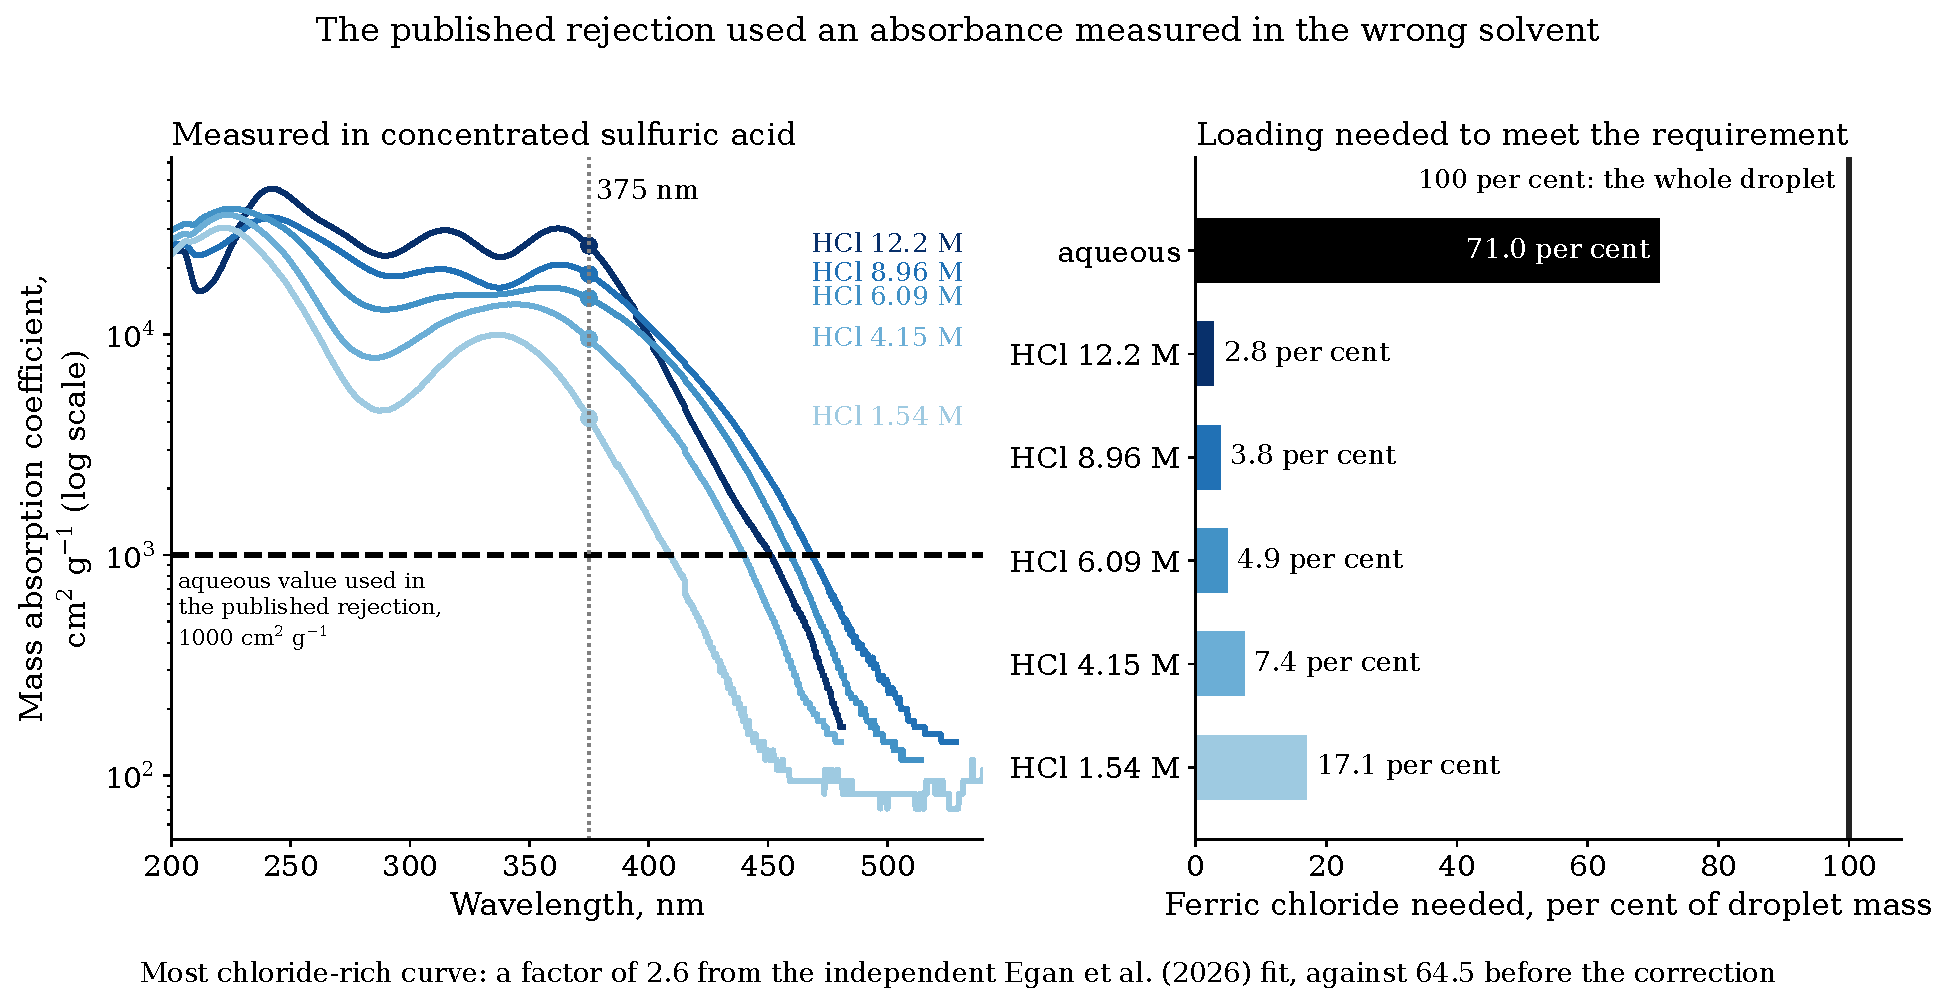
\includegraphics[width=\textwidth]{F17_E14_ferric-chloride-correction_ch6_s16.pdf}
  \caption[Ferric chloride in hydrochloric acid and the loading each curve needs (Experiment~14)]{Ferric chloride in hydrochloric acid at five strengths (left, read from Egan
    et al.~\cite{egan2025lab}) and the loading each needs as a share of the droplet mass
    (right), against the aqueous value of the published rejection (Experiment~14). The
    curves are those of their Figure~5a. Keys
    \texttt{e14.ClA.*} to \texttt{e14.ClE.*} and \texttt{e14.factor\_to\_fit\_after}.}
  \label{fig:F17}
\end{figure}

\textbf{Result.} In these solutions, ferric chloride absorbs 4.164 to 25.192 times more
strongly at 375~nm than the aqueous value (\texttt{e14.ratio\_lo},
\texttt{e14.ratio\_hi}). The loading needed falls from 1.278~kg per litre to between
0.0507 and 0.3069, that is from 71.0\% of the droplet mass to between 2.82\% and 17.05\%
(\texttt{e14.ClA.pct\_of\_droplet}, \texttt{e14.ClE.pct\_of\_droplet};
Figure~\ref{fig:F17}). If ferric chloride in the droplets absorbs as it does in any of
these solutions, the rejection does not survive: even the weakest curve leaves it a
plausible minor component. The answer is a range because the iron forms several chloride
complexes whose shares depend on the chloride available, and how much chloride the
droplets hold is not settled here. Table~\ref{tab:e14} shows the trend: the more hydrochloric acid in
the solution, the more strongly ferric chloride absorbs at 375~nm and the less of it is
needed.

\begin{table}[htbp]
  \centering
  \caption[The five ferric chloride curves at 375~nm (Experiment~14)]{The five ferric chloride curves of Egan et al.~\cite{egan2025lab} at 375~nm,
    and the loading each needs by Equation~\eqref{eq:loading} (Experiment~14). Molar
    $\varepsilon$ in litres per mole per centimetre, mass $\varepsilon$ in square
    centimetres per gram; share of the droplet's own mass. Keys
    \texttt{e14.<curve>.hcl\_M}, \texttt{.eps\_molar}, \texttt{.eps\_mass},
    \texttt{.loading\_kg\_per\_L} and \texttt{.pct\_of\_droplet}.}
  \label{tab:e14}
  \footnotesize
  \setstretch{1.0}
  \begin{tabular}{lccccc}
    \toprule
    Curve & HCl (mol/L) & $\varepsilon$, molar & $\varepsilon$, mass & Loading (kg/L) &
      Share (\%) \\
    \midrule
    Cl~A & 12.20 & 4086.212 & 25191.806 & 0.0507 & 2.82 \\
    Cl~B & 8.96 & 3036.595 & 18720.842 & 0.0683 & 3.79 \\
    Cl~C & 6.09 & 2362.116 & 14562.626 & 0.0878 & 4.88 \\
    Cl~D & 4.15 & 1546.601 & 9534.912 & 0.1340 & 7.45 \\
    Cl~E & 1.54 & 675.439 & 4164.130 & 0.3069 & 17.05 \\
    \bottomrule
  \end{tabular}
\end{table}

The correction also brings two 2026 papers that do not cite each other closer. The
preprint of Egan et al., not peer reviewed, fits 1.0 to 1.2~wt\% ferric chloride in the
smallest droplets to the MESSENGER spectrum~\cite{egan2026}. The most chloride-rich curve
here needs 2.82\%, a factor of 2.6 from the middle of that range
(\texttt{e14.factor\_to\_fit\_after}), against 64.5 before. The two figures still rest on
different assumptions: Spacek et al.\ spread the absorber through two droplet sizes in a
layer near the cloud top, while the preprint puts it in the smallest droplets only, which
also reach higher into the haze. Spacek et al.\ note that either change would alter their
requirement, in opposite directions~\cite{spacek2026}, so the remaining factor of 2.6 is
not a contradiction, but it is not yet explained.

\textbf{What Experiment 14 does not claim.} It corrects one input to another group's
argument. It does not identify the absorber, and nothing in it measures Venus. The
laboratory spectra were taken far more dilute than these loadings and are scaled in a
straight line, as Spacek et al.\ also do. Above all, ferric chloride has not been tested
on altitude, the test that decided Experiment~9, because it has no chemistry in the model
and so cannot be placed by it. That test belongs to Phase~2 (Chapter~9).

% ===========================================================================
\section{What Experiments 8 to 14 establish}
\label{sec:e814-summary}

\begin{itemize}
  \item Placement matters more than spectral shape, 7.34 against 4.95, and shape matters
    only where the absorber overlaps the responding layer.
  \item Placed by the model's own chemistry, the closest gas-phase candidate falls out of
    the response band and becomes radiatively the same as no absorber.
  \item Two runs that should agree give radiation fields that differ by 0.0017\% of the
    change they make, but change the SO abundance in the band by 0.7384\% and 2.5278\%
    from the same baseline. An apparent
    fingerprint was linear response and has been withdrawn.
  \item No species the model can represent passes amount, placement and spectrum together,
    and the three tests disagree about which comes closest.
  \item At 375~nm the proposed iron and sulfur minerals cannot absorb enough even as
    pure solids. Ferric chloride, rejected on an aqueous measurement, becomes a plausible
    minor component if it absorbs in the droplets as it does in hydrochloric acid, but
    its altitude is untested.
\end{itemize}
